% v1.0 (c) | Copyright 2024 Daniel E. Janusch

% this file is licensed by https://raw.githubusercontent.com/drizzt536/files/main/LICENSE
% and must be copied IN ITS ENTIRETY under penalty of law.

% run with shell escape
% I compile with my Sublime Text build tool, which uses latexmk.

\newcommand \hpx [1]{\hspace{#1px}}
\newcommand \nhpx [1]{\hspace{-#1px}}

\newcommand \final {\mathrm{final}}
\newcommand \clamp {\mathrm{clamp}}
\newcommand \vvec {\nhpx 1 \vec{\hpx 1 v}}
\newcommand \uvec {\nhpx 1 \vec{\hpx 1 u}}

\newcommand \unchckdBox {\raisebox{-1px}{$\square$}\hspace{-8.2px}\raisebox{1px}{\phantom \checkmark}~\,}
\newcommand \checkedBox {\raisebox{-1px}{$\square$}\hspace{-8.2px}\raisebox{1px}\checkmark~\,}

\documentclass[12pt]{article}

\usepackage[
	top    = 0.50in,
	left   = 1.25in,
	right  = 1.25in,
	bottom = 1.00in,
]{geometry}

\usepackage{
	amsmath,
	amssymb,
	latexsym,
	xcolor,
	minted,
	graphicx,
	enumitem,
	hyperref,
	xurl
}

\definecolor{lightgray}{RGB}{170, 170, 170} % #AAA
\definecolor{keyword}{RGB}{198, 149, 198}   % #C695C6
\definecolor{operator}{RGB}{249, 123, 87}   % #F97B57
\definecolor{variable}{RGB}{216, 222, 233}  % #D8DEE9
\definecolor{function}{RGB}{102, 153, 204}  % #69C

\color{lightgray}
\pagecolor{black}

\begin{document}

\newgeometry{
	top    = 0.00in,
	left   = 1.25in,
	right  = 1.25in,
	bottom = 1.00in,
}

\title{EGR 115 Final Project Proposal {\bf–} SVG Inverter}
\author{Daniel E. Janusch}
\date{November 12, 2024}
\maketitle

\vspace{-30px}
\section{Input/Output Examples}

\begin{figure}[ht]
	\centering
	\begin{minipage}[b]{0.441\textwidth}
		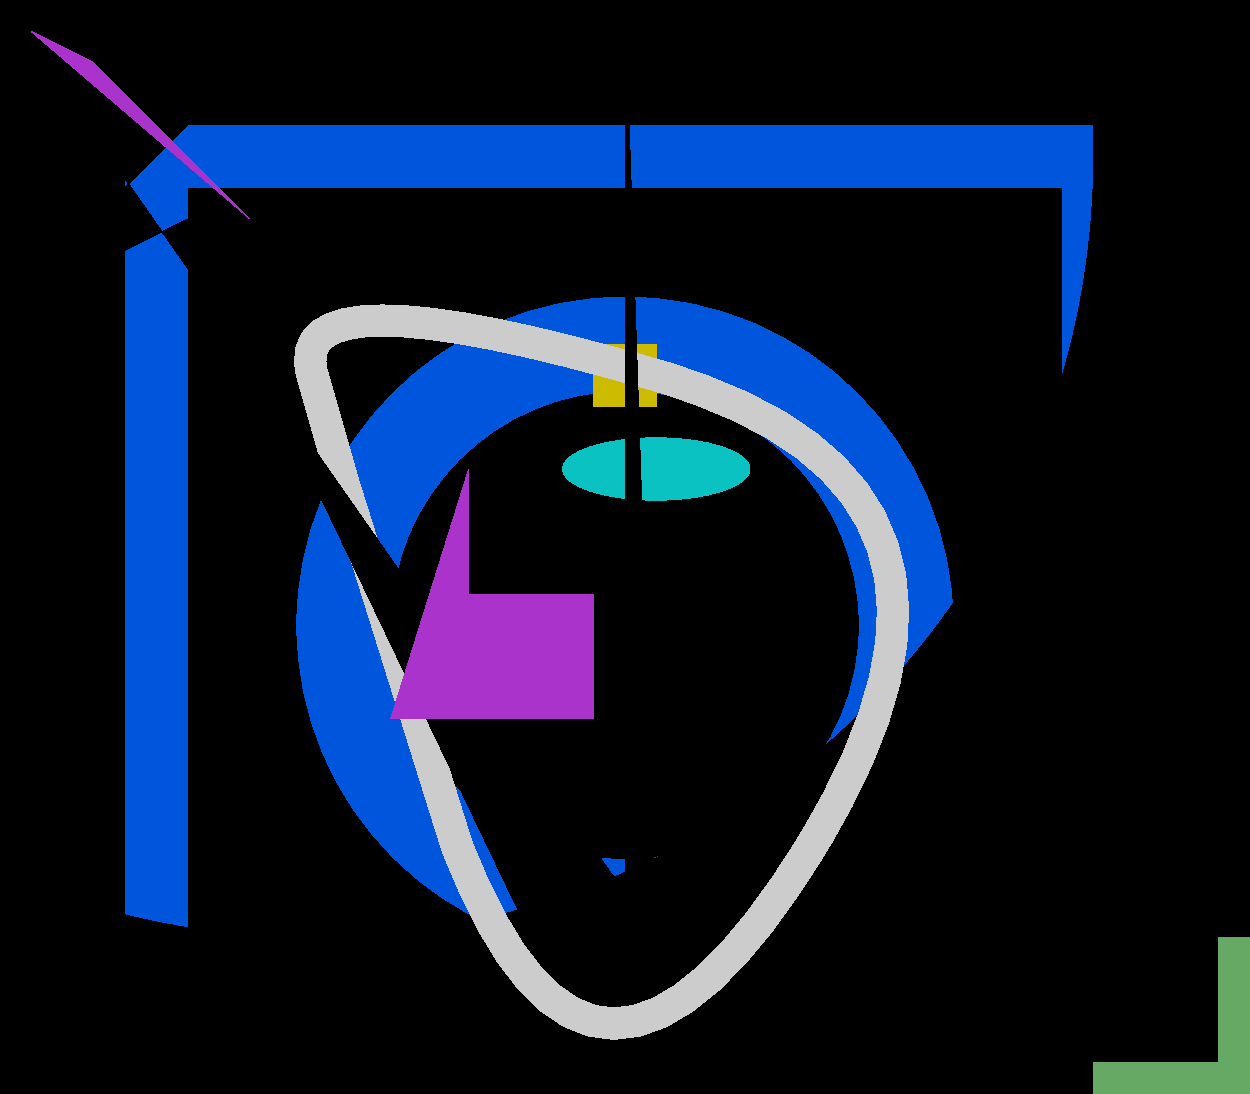
\includegraphics[width=\textwidth]{./pdf/ex1-dark.pdf}
		\caption{Ex 1. Original SVG}
	\end{minipage}
	\hfill
	\begin{minipage}[b]{0.441\textwidth}
		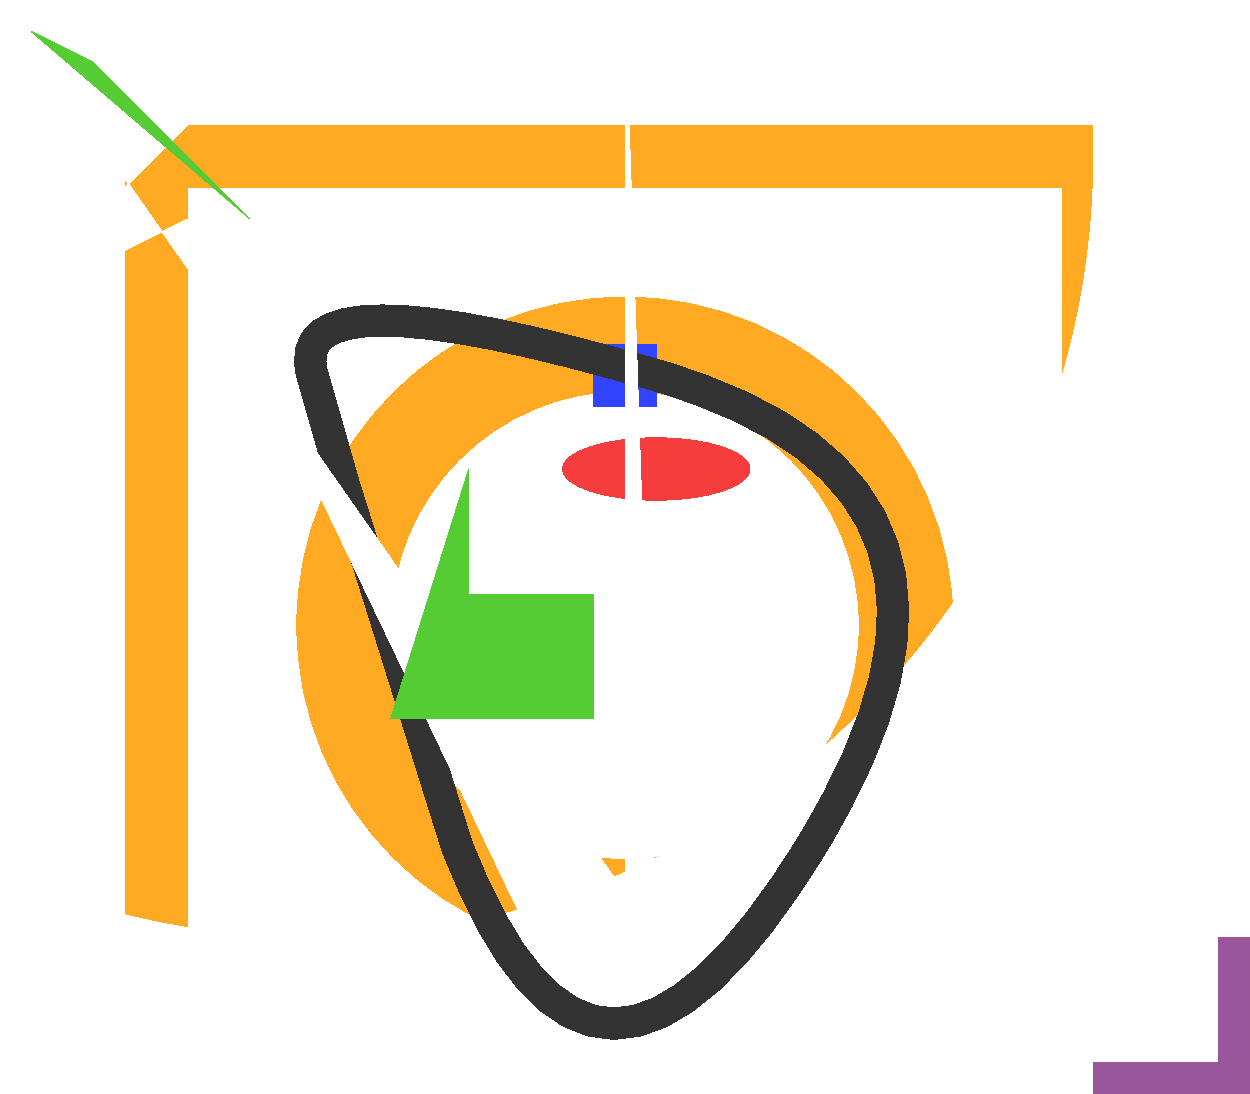
\includegraphics[width=\textwidth]{./pdf/ex1-light.pdf}
		\caption{Ex 1. Inverted SVG}
	\end{minipage}
\end{figure}

\begin{figure}[ht]
	\centering
	\begin{minipage}[b]{0.441\textwidth}
		
\includegraphics[width=\textwidth]{./pdf/ex3-light.pdf}
		\caption{Ex 2. Original SVG}
	\end{minipage}
	\hfill
	\begin{minipage}[b]{0.441\textwidth}
		
\includegraphics[width=\textwidth]{./pdf/ex3-dark.pdf}
		\caption{Ex 2. Inverted SVG}
	\end{minipage}
\end{figure}

\pagebreak
\restoregeometry

\section{Program Overview}

\subsection{Program Psueocode}

\begin{verbatim}
print the help text if requested

if no file was given, throw an error

read in the file content to a variable

test if each <rect> has the same dimensions as the SVG
add a background <rect> to the SVG if there wasnt one already

invert all the stroke colors
invert all the fill colors

find all the IDs of images referenced in <use> tags within the <mask> tag
find all the inline images within <mask> tags

for each <image> in the SVG
    if the image is defined or referenced in a <mask>
        continue

    invert the image using ImageMagick and update the SVG

trim and output the content, either to a file or to stdout.
\end{verbatim}

\subsection{MATLAB Capabilities Used}

\begin{itemize}[label={}]
	\item \checkedBox conditionals (e.g. \textcolor{keyword}{\texttt{if}}, \textcolor{keyword}{\texttt{switch}})
	\item \checkedBox loops (e.g. \textcolor{keyword}{\texttt{for}}, \textcolor{keyword}{\texttt{while}})
	\item \checkedBox matrix and array operations$^*$ (e.g. \textcolor{operator}{\texttt{.*}}, \textcolor{operator}{\texttt{.\^{}}}, \textcolor{operator}{\texttt\textbackslash})
	\item \checkedBox string and character arrays and operations
	\item \checkedBox data I/O (e.g. file or stdin/stdout)
	\item \unchckdBox visualization (plots)
	\item \checkedBox boolean operations (e.g. \textcolor{operator}{\texttt{||}}, \textcolor{operator}{\texttt{\&\&}})
	\item \checkedBox built-in functions (e.g. \textcolor{function}{\texttt{struct}}, \textcolor{function}{\texttt{extractBetween}}, \textcolor{function}{\texttt{regexpi}})
\end{itemize}

\vfill {\scriptsize $^*$only if the additions are made, discussed on the next page}

\pagebreak

\section{Possible Project Additions}

I could use some kind of continuous map like a vector function or matrix
transformation instead of just inverting the colors. I could also rasterize the
inverted image and analyze and plot the color distribution, which would mark off
the visualization aspect of MATLAB. Using a color transformation matrix wouldn't
allow for all linear transformations, so this will be used instead:

\vspace{3px}
$C_2 =\begin{bmatrix}
	r_0 \\ g_0 \\ b_0
\end{bmatrix} + \begin{bmatrix}
	a \\ b \\ c
\end{bmatrix} \! \odot \! \begin{bmatrix}
	R \\ G \\ B
\end{bmatrix} = \begin{bmatrix}
	r_0 + a R \\ g_0 + b G \\ b_0 + c B
\end{bmatrix}$ given $\begin{bmatrix}
	R \\ G \\ B
\end{bmatrix}$ as the input.

\vspace{3px}
and either $C_\final = \text{clamp}(C_2, \textbf[0~\,255\textbf])$
or $C_\final = C_2 \, \text{mod} \, 256$

$\uvec \odot \vvec$ is the Hadamard Product of $\uvec$ and $\vvec$ (\texttt{\textcolor{variable}u \textcolor{operator}{.*} \textcolor{variable}v}).

\section{Appendix}

\noindent {\footnotesize Example 1 original:}

\begin{minted}[fontsize=\scriptsize, linenos]{xml}
<?xml version="1.0" encoding="UTF-8"?>
<svg xmlns="http://www.w3.org/2000/svg" width="800" height="700" viewBox="0 0 40 35">
    <rect width="40" height="35" fill="#000"/>
    <rect width="30" height="30" x="5" y="5" stroke-width="2" fill-opacity="0" stroke="#05d"/>
    <circle cx="20" cy="20" r="9" stroke-width="3" fill-opacity="0" stroke="#05d"/>
    <circle cx="10" cy="5" r="34" stroke-width="18" fill-opacity="0" stroke="#000"/>
    <rect x="19" y="11" width="2" height="2" fill="rgb(204, 187, 0)"/>
    <ellipse cx="21" cy="15" rx="3" ry="1" fill="hsl(180, 90%, 40%)"/>
    <path d="M 11 15.5 T 10 12, 21 12, 26 27, 14.6 27 Z" stroke="#ccc" fill="none"/>
    <polygon points="0 0 10 0 0 10 6 7 17 30 20 30 20 0 21 30" fill="#000"/>
    <path d="M 1 1 l 2 1 5 5 z M 15 15 v 4 h 4 v 4 h -6.5" fill="#a3c"/>
    <polygon points="40,35  40,30  39,30  39,34  35,34  35,35" fill="#65a965"/>
</svg>
\end{minted}

\noindent {\footnotesize Example 1 final:}

\begin{minted}[fontsize=\scriptsize, linenos]{xml}
<?xml version="1.0" encoding="UTF-8"?>
<svg xmlns="http://www.w3.org/2000/svg" width="800" height="700" viewBox="0 0 40 35">
    <rect width="40" height="35" fill="#fff"/>
    <rect width="30" height="30" x="5" y="5" stroke-width="2" fill-opacity="0" stroke="#fa2"/>
    <circle cx="20" cy="20" r="9" stroke-width="3" fill-opacity="0" stroke="#fa2"/>
    <circle cx="10" cy="5" r="34" stroke-width="18" fill-opacity="0" stroke="#fff"/>
    <rect x="19" y="11" width="2" height="2" fill="rgb(51, 68, 255)"/>
    <ellipse cx="21" cy="15" rx="3" ry="1" fill="hsl(0, 90%, 60%)"/>
    <path d="M 11 15.5 T 10 12, 21 12, 26 27, 14.6 27 Z" stroke="#333" fill="none"/>
    <polygon points="0 0 10 0 0 10 6 7 17 30 20 30 20 0 21 30" fill="#fff"/>
    <path d="M 1 1 l 2 1 5 5 z M 15 15 v 4 h 4 v 4 h -6.5" fill="#5c3"/>
    <polygon points="40,35  40,30  39,30  39,34  35,34  35,35" fill="#9a569a"/>
</svg>
\end{minted}

\vfill
{\scriptsize Example 2 is derived from \url{https://upload.wikimedia.org/wikipedia/commons/7/7b/Adobe_Systems_logo_and_wordmark.svg}}

\end{document}
